% !TEX root = ../main.tex
\section{Q14: Informativeness-prinsippet -- kontrollerbarhed, risikodeling, presisjon, risikopræmie}\label{q:14}

\begin{quote}
\emph{Redegør for Informativeness-princippet i relation til design af kontrakter og kompensation. Følgende forhold og begreber forventes inddraget: a) kontrollerbarhed, b) risikodeling, c) målingers præcision, d) risikopræmie.}
\end{quote}

\subsection*{Svar (kort)}
Informativeness-prinsippet (Holmström 1979) sier at et signal $y$ bør inkluderes i kontrakten hvis og bare hvis det er statistisk informativt om agentens innsats -- dvs.\ at det endrer posterior for $e$ gitt det primære målet $Q$. Prinsippet binder de fire delspørsmålene sammen: (a) controllability er et \emph{spesialtilfelle} -- informativeness er bredere, fordi ukontrollerbare mål kan likevel være informative; (b) mer informative signaler forbedrer risikodelingen ved å senke effektiv støy; (c) presise mål (lav $\sigma^2$) er mer informative og bør vektes høyere ($\beta$ opp); (d) risikopremien $RP = \tfrac{r}{2}\beta^2\sigma^2$ synker når signaler filtrerer bort støy. [SLIDE]

\subsection*{Relevante teorier (kort)}

\paragraph{\thref{informativeness-principle}{Informativeness-prinsippet}\quad\STwo/\SThree}
Holmströms tilstrekkelighets\-kriterium: inkludér signal $y$ i kontrakten $\Leftrightarrow$ $f(Q|e,y)\neq f(Q|e)$ for noen $(Q,y)$. Kontrakt utvides til $W=W_0+\beta_1 Q + \beta_2 y$. Effekten: lavere effektiv varians $\sigma^2_{\text{eff}} < \sigma^2$, dermed lavere risikopremie for gitt insentivnivå, eller sterkere insentiver for gitt risikopremie. Sufficient statistic-poenget: hvis $Q$ allerede fanger all informasjon om $e$, skal $y$ \emph{ikke} brukes. [SLIDE]

\paragraph{\thref{controllability-principle}{(a) Controllability-prinsippet}\quad\STwo}
Lederen skal kun evalueres på det hun kontrollerer. Men informativeness \emph{generaliserer} dette: et ukontrollerbart mål (f.eks.\ bransjeavkastning, oljepris) kan \emph{forbedre} kontrakten hvis det filtrerer ut felles sjokk fra agentens mål. Controllability er nødvendig i snever forstand (ikke straff for eksogene sjokk), men informative mål som er ukontrollerbare er likevel verdifulle som filtreringsinstrumenter. [SLIDE]

\paragraph{\thref{risk-sharing}{(b) Risikodeling}\quad\SThree}
Risikoavers agent + risikonøytral prinsipal $\Rightarrow$ first-best er fast lønn. Men \thref{moral-hazard}{moral hazard} krever $\beta>0$ for å vri innsats $\Rightarrow$ agenten bærer risiko $\Rightarrow$ risikopremie. Informativeness forbedrer trade-offen: med mer informative signaler kan man oppnå \emph{samme} innsatsnivå med \emph{lavere} risiko for agenten, eller \emph{høyere} innsats med \emph{samme} risiko. Risikodelingen blir Pareto-bedre. [SLIDE]

\paragraph{\thref{incentive-coefficient}{(c) Målingers presisjon og (d) risikopremie}\quad\STwo/\SThree}
Presisjon = invers varians: høy presisjon $\Rightarrow$ lav $\sigma^2$ $\Rightarrow$ høyere $\beta^*$ (\thref{incentive-coefficient}{$\beta^* = 1/(1+r\sigma^2 c''/\alpha^2)$}). Risikopremien $RP = \tfrac{r}{2}\beta^2\sigma^2$ er stigende i støy -- upresise mål er dyre å bruke som insentivgrunnlag. Informativeness-prinsippet sier: legg til signaler som øker presisjonen (senker effektiv $\sigma^2$), og unngå signaler som bare tilfører støy. Relative prestasjonsmål (\thref{absolute-vs-relative-performance}{rTSR}) er det viktigste eksemplet: peer-avkastning filtrerer felles markedssjokk og øker presisjonen av det individuelle signalet. [SLIDE/BOK]

\subsection*{Illustrasjon -- informativeness-prinsippet}

\begin{figure}[h]
\centering
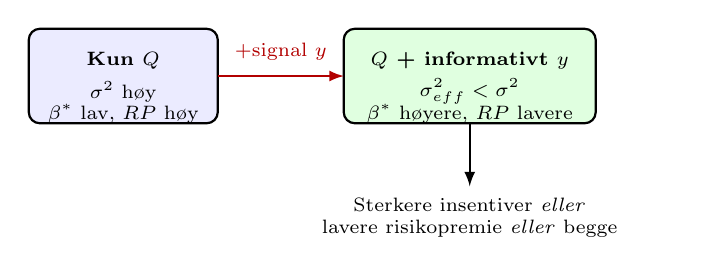
\begin{tikzpicture}[>=latex, scale=0.8, every node/.style={font=\small}]
  % Q bare
  \draw[thick, rounded corners, fill=blue!8] (0,3.0) rectangle (3.0,4.5);
  \node[font=\bfseries\scriptsize] at (1.5,4.0) {Kun $Q$};
  \node[font=\scriptsize] at (1.5,3.5) {$\sigma^2$ høy};
  \node[font=\scriptsize] at (1.5,3.15) {$\beta^*$ lav, $RP$ høy};
  % Q + y
  \draw[thick, rounded corners, fill=green!12] (5.0,3.0) rectangle (9.0,4.5);
  \node[font=\bfseries\scriptsize] at (7.0,4.0) {$Q$ + informativt $y$};
  \node[font=\scriptsize] at (7.0,3.5) {$\sigma^2_{\text{eff}} < \sigma^2$};
  \node[font=\scriptsize] at (7.0,3.15) {$\beta^*$ høyere, $RP$ lavere};
  % Arrow
  \draw[->, thick, red!70!black] (3.0,3.75) -- (5.0,3.75);
  \node[above, font=\scriptsize, red!70!black] at (4.0,3.85) {+signal $y$};
  % Resultat
  \draw[->, thick] (7.0,3.0) -- (7.0,2.0);
  \node[font=\scriptsize, text width=5cm, align=center] at (7.0,1.5) {Sterkere insentiver \emph{eller}\\lavere risikopremie \emph{eller} begge};
\end{tikzpicture}
\caption{Informativeness: tillegg av informativt signal $y$ senker effektiv $\sigma^2$ og forbedrer insentiv-risiko-trade-offen. [SLIDE/BOK]}
\end{figure}

\subsection*{Kobling mellom de fire delspørsmålene}

\begin{center}
\renewcommand{\arraystretch}{1.15}
\begin{tabular}{@{}p{3.2cm}p{4.5cm}p{5.5cm}@{}}
\toprule
\textbf{Begrep} & \textbf{Rolle i modellen} & \textbf{Kobling til informativeness} \\
\midrule
(a) Kontrollerbarhet & Mål det agenten kan styre & Informativeness er \emph{bredere}: ukontrollerbare mål kan likevel filtrere støy \\
(b) Risikodeling & $\beta>0 \Rightarrow$ agenten bærer risiko & Bedre signaler $\Rightarrow$ bedre risikodeling for gitt innsats \\
(c) Presisjon & Invers varians av signal & Presise mål er mer informative $\Rightarrow$ høyere $\beta^*$ \\
(d) Risikopremie & $RP = \tfrac{r}{2}\beta^2\sigma^2$ & Lavere effektiv $\sigma^2 \Rightarrow$ lavere $RP$ \\
\bottomrule
\end{tabular}
\end{center}

\subsection*{Slide-figur fra BSZ kap.\ 15}

\begin{figure}[h]
  \centering
  
\includegraphics[width=0.55\linewidth]{BSZ_kap_15_2026/by_slide/slide_014/BSZ_kap_15_2026_slide_014_asset_01_image3.png}
  \caption{Principal-agent-modellens notasjon fra BSZ kap.\ 15: $Q=\alpha e + \mu$, $W=W_0+\beta Q$. Informativeness-prinsippet utvider denne rammen med tilleggssignaler. [SLIDE -- BSZ kap.\ 15, slide 14]}
\end{figure}

\subsection*{Real-world eksempler}

\textbf{Eks.~1 -- Equinor CEO-kompensasjon (relativ Total Shareholder Return).}\quad [EKS]
Equinors LTI-program bruker \emph{relative TSR} mot en peer-gruppe av internasjonale energiselskaper (Shell, BP, TotalEnergies). Oljepris er et ukontrollerbart signal -- men det er \emph{informativt}: ved å trekke fra peer-gruppens avkastning filtreres felles oljeprisssjokk ut, og bonusen reflekterer den delen av avkastningen som skyldes konsernsjefens beslutninger. Informativeness-prinsippet er direkte grunnlaget: peer-TSR er et informativt signal ($y$) som senker effektiv $\sigma^2$ og tillater sterkere insentiver ($\beta$) uten uakseptabel risikopremie.

\textbf{Eks.~2 -- Norsk sykehuslege (kun subjektive mål), sammenligning.}\quad [EKS]
En sykehuslege evalueres i praksis kun subjektivt (avdelingsleders helhetsvurdering). Pasientutfall (helbredelse, overlevelse) er et upresist mål ($\sigma^2$ enorm -- avhenger av pasientens helsetilstand, komorbiditet). Informativeness-prinsippet tilsier at man \emph{bør} legge til informative signaler: prosessmål (etterlevelse av protokoller), volumjusterte utfallsmål, peer-sammenligning (case-mix-justert dødelighet). Men informasjonskostnaden er høy, og multitasking-problemet gjør at sterke insentiver på målt dimensjon vrir bort fra umålt omsorgskvalitet. Kontrasten med Equinor: i energibransjen er signalene (aksjekurs, oljepris) billige og informative; i helsesektoren er de dyre og upresise -- forskjellen forklarer ulik kontraktsdesign.

\subsection*{Kobling til Mærsk Power-to-X}
PtX-divisionens ledelse illustrerer alle fire aspekter: [CASE]
\begin{itemize}\setlength{\itemsep}{2pt}
\item \textbf{(a) Kontrollerbarhet:} Lederen kontrollerer prosjektgjennomføring men ikke elpris eller H$_2$-etterspørsel.
\item \textbf{(b) Risikodeling:} Stor $\sigma^2$ fra eksogene markeder $\Rightarrow$ lav $\beta$ på topplinjeresultat for å begrense risikopremie.
\item \textbf{(c) Presisjon:} Milestones (FID, anlegg ferdig, OPEX-budsjett) er presise og kontrollerbare $\Rightarrow$ kan bære høyere $\beta$.
\item \textbf{(d) Risikopremie:} Ved å bruke milestones + peer-benchmark (Ørsted, Air Liquide) senkes $\sigma^2_{\text{eff}}$ $\Rightarrow$ lavere $RP$.
\end{itemize}

\subsection*{Fallgruber}
\begin{itemize}\setlength{\itemsep}{2pt}
\item Presentere de fire begrepene som uavhengige -- de bindes sammen av informativeness-prinsippet.
\item Forveksle informativeness med controllability -- informativeness er \emph{bredere}; ukontrollerbare mål kan være informative.
\item Glemme sufficient statistics-poenget: ikke alle signaler er nyttige; noen tilfører bare støy.
\item Ikke nevne formelen: $\beta^* = 1/(1+r\sigma^2 c''/\alpha^2)$ -- den kobler presisjon og risikopremie direkte.
\item Bare abstrakt teori uten eksempel på relative mål (rTSR, peer-justering).
\item Glemme multitasking-begrensningen (Holmström--Milgrom): sterke insentiver på informative men ensidige mål vrir innsats.
\end{itemize}

\subsection*{Håndskrivbar disposisjon (15-min forberedelse)}
\begin{itemize}\setlength{\itemsep}{2pt}
\item \textbf{Tese:} Informativeness-prinsippet (Holmström 1979) er det overordnede rammeverket; (a)--(d) er konsekvenser/aspekter av det.
\item \textbf{Definisjon:} $y$ informativt $\Leftrightarrow$ endrer posterior for $e$ gitt $Q$. Sufficient statistic: inkluder $y$ \emph{bare} hvis det tilfører informasjon.
\item \textbf{(a) Kontrollerbarhet:} spesialtilfelle; informativeness er bredere (ukontrollerbare mål kan filtrere).
\item \textbf{(b) Risikodeling:} bedre signaler $\Rightarrow$ Pareto-bedre risk-sharing for gitt innsats.
\item \textbf{(c) Presisjon:} lav $\sigma^2$ $\Rightarrow$ høyere $\beta^*$. Formel: $\beta^*=1/(1+r\sigma^2 c''/\alpha^2)$.
\item \textbf{(d) Risikopremie:} $RP=\tfrac{r}{2}\beta^2\sigma^2$; lavere eff.\ $\sigma^2 \Rightarrow$ lavere $RP$.
\item \textbf{Kobling:} tabell som knytter a-b-c-d til informativeness.
\item \textbf{Hovedeksempel:} Relativ TSR (rTSR) -- peer-signal filtrerer markedssjokk.
\item Eks.\ 1: Equinor CEO + rTSR. Eks.\ 2: Norsk sykehuslege (upresise mål, subjektiv evaluering).
\item Case: Mærsk PtX -- milestones + peer-benchmark som informative signaler.
\item \textbf{Kritikk:} multitasking (HM 1991), kognitiv overbelastning, informasjonskostnad.
\item Søyle: \STwo\ (måldesign) + \SThree\ (kontraktsdesign).
\end{itemize}
